\chapter{GPIO Inputs and Interrupt Handling}

\section*{Learning Objectives}
After completing this experiment, you will be able to:
\begin{itemize}[nosep]
  \item Configure GPIO inputs with digital enable and internal pull resistors.
  \item Read switches via polling with software debouncing (typ. 20\,ms).
  \item Configure edge-triggered GPIO interrupts and write minimal ISRs.
  \item Enable and manage interrupts in the NVIC (IRQ mapping, ISER).
  \item Unlock and configure protected pins (PF0/NMI) for general-purpose use.
\end{itemize}


\section*{Experiment Overview}
This experiment extends GPIO functionality to inputs and introduces interrupt-driven programming. You will configure GPIO pins to read mechanical switches using both polling and interrupt approaches, implement software debouncing techniques, write interrupt service routines, and enable GPIO interrupts in the NVIC. By the end of this lab, you will understand how to implement both polling and interrupt-driven input handling, and write responsive embedded applications that react to external events in real time.

\newpage


\section{Theoretical Background}

\subsection{GPIO Input Configuration}

In the previous experiment, GPIO pins were configured as outputs to control LEDs. In this experiment, we configure GPIO pins as \textbf{inputs} to read the state of external devices such as switches, buttons, and sensors.

When a GPIO pin is configured as an input, the microcontroller reads the voltage level on the pin and interprets it as a logic '0' (low, typically 0V) or logic '1' (high, typically 3.3V). The pin's digital input buffer must be enabled, and the pin must be connected to a defined voltage level to avoid floating states.

\subsubsection{Input Pin Requirements}

For reliable digital input operation, three conditions must be met:
\begin{itemize}[nosep]
  \item \textbf{Direction}: The pin must be configured as an input (bit cleared in \texttt{GPIODIR}).
  \item \textbf{Digital Enable}: The digital input buffer must be enabled (bit set in \texttt{GPIODEN}).
  \item \textbf{Defined Logic Level}: The pin must be connected to a valid logic level (not floating).
\end{itemize}

\noindent
If a pin is left floating (not connected to a defined voltage), it can pick up electrical noise and produce random or unstable readings. To prevent this, pins are typically connected to either power (\texttt{VCC}) or ground (\texttt{GND}) through a resistor, or the microcontroller's internal pull-up or pull-down resistors can be enabled.

\subsubsection{Pull-Up and Pull-Down Resistors}
\label{sec:pull-resistors}

Digital inputs must not be left floating: an undefined voltage can produce random logic reads. A pull resistor defines the idle (no-press) level of a switch input.

\paragraph{Pull-Up (active-low)}
A \textbf{pull-up} connects the pin weakly to $V_{CC}$, so the idle level is logic~1. Pressing the switch drives the pin to GND $\rightarrow$ logic~0.

\paragraph{Pull-Down (active-high)}
A \textbf{pull-down} connects the pin weakly to GND, so the idle level is logic~0. Pressing the switch drives the pin to $V_{CC}$ $\rightarrow$ logic~1.


\begin{figure}[H]
    \centering
    % Requires \usepackage{circuitikz}, \usepackage{amsmath}, \usepackage{subcaption}
    \begin{circuitikz}[american, scale=0.95, transform shape,
        % Define styles for clarity
        input/.style={thick, ->},
        state_high/.style={draw=black!60!black, thick},
        state_low/.style={draw=black!60!black, thick}
    ]

    % --- Pull-Up Circuit (Left Subfigure) ---
    \begin{scope}[shift={(0,0)}]
        \draw[state_high] (0, 4) node[above] {$V_{CC}$} coordinate (VCC_PU)
            to[R, l=$R_{PU}$] (0, 2.5) coordinate (Input_PU);

        % Connection to MCU Input
        \draw[input] (Input_PU) -- ++(1.5, 0) node[right] {$\substack{\text{MCU Input} \\ \text{(Default High)}}$};

        % Switch to Ground (Active Low)
        \draw (Input_PU) to[short, *-] (-1.5, 2.5) coordinate (SW_Top);
        \draw[state_low] (SW_Top) to[nopb, l={SW}] (-1.5, 0) coordinate (SW_Bottom);
        \draw (SW_Bottom) -- (0, 0) node[ground] {} node[below] {};

        \node at (0, 5.2) {\textbf{A) Pull-Up Configuration}};
    \end{scope}

    % --- Pull-Down Circuit (Right Subfigure) ---
    \begin{scope}[shift={(7,0)}]
        \draw (0, 4) node[above] {$V_{CC}$} coordinate (VCC_PD);

        % Switch to VCC (Active High)
        \draw (VCC_PD) to[short, *-] (-1.5, 4) coordinate (SW_Top);
        \draw[state_high] (SW_Top) to[nopb, l={SW}] (-1.5, 1.5) coordinate (SW_Bottom);

        \draw (SW_Bottom) to[short, *-] (0, 1.5) coordinate (Input_PD);

        % Resistor to Ground
        \draw[state_low] (Input_PD) to[R, l_=$R_{PD}$] (0, 0) node[ground] {} node[below] {};

        % Connection to MCU Input
        \draw[input] (Input_PD) -- ++(1.5, 0) node[right] {$\substack{\text{MCU Input} \\ \text{(Default Low)}}$};

        \node at (0, 5.2) {\textbf{B) Pull-Down Configuration}};
    \end{scope}

    \end{circuitikz}
    \caption{Pull-Up and Pull-Down Resistor Configurations for Switch Inputs}
    \label{fig:pull_circuits_improved}
\end{figure}

\paragraph{Internal Resistors (TM4C123)}
TM4C123 GPIO pins include configurable \textbf{internal} pull resistors:
\begin{itemize}[noitemsep, topsep=2pt]
  \item \texttt{GPIOPUR} — Pull-Up Select (enable bit = pull-up on that pin)
  \item \texttt{GPIOPDR} — Pull-Down Select (enable bit = pull-down on that pin)
\end{itemize}
Do not enable both on the same pin. On the LaunchPad, SW1 (PF4) and SW2 (PF0) short to GND when pressed, so enable \textbf{pull-ups} (\texttt{GPIOPUR}) to make them active-low (read 0 when pressed, 1 when released).

\subsection{Switch Bouncing and Debouncing}

When a mechanical switch or button is pressed or released, the metal contacts inside do not make or break contact cleanly. Instead, they \textbf{bounce} — rapidly making and breaking contact multiple times before settling into a stable state. This bouncing typically lasts 5-30 milliseconds.

\begin{figure}[H]
\centering
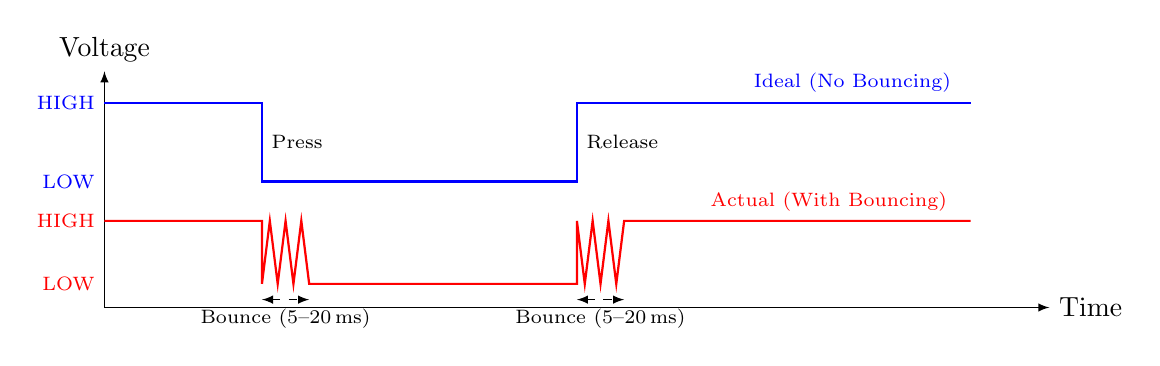
\begin{tikzpicture}[x=1cm,y=1cm,>=latex]
  % Axes
  \draw[->] (0,0) -- (12,0) node[right]{Time};
  \draw[->] (0,0) -- (0,3) node[above]{Voltage};

  % --- Ideal signal lane (upper) ---
  % Levels for the upper lane
  \def\HIGHU{2.6}
  \def\LOWU{1.6}
  % Ideal (no bounce)
  \draw[thick, blue]
    (0,\HIGHU) -- (2,\HIGHU)
    -- (2,\LOWU)
    -- (6,\LOWU)
    -- (6,\HIGHU)
    -- (11,\HIGHU);
  \node[blue] at (9.5,2.85) {\scriptsize Ideal (No Bouncing)};
  \node[blue, anchor=east] at (0,\HIGHU) {\scriptsize HIGH};
  \node[blue, anchor=east] at (0,\LOWU) {\scriptsize LOW};

  % --- Actual signal lane (lower) ---
  % Levels for the lower lane
  \def\HIGHL{1.1}
  \def\LOWL{0.3}
  % Actual with bounce (press and release)
  \draw[thick, red]
    (0,\HIGHL) -- (2,\HIGHL)
    % Press bounce
    -- (2,\LOWL)
    -- (2.10,\HIGHL)
    -- (2.20,\LOWL)
    -- (2.30,\HIGHL)
    -- (2.40,\LOWL)
    -- (2.50,\HIGHL)
    -- (2.60,\LOWL)
    -- (6,\LOWL)
    % Release bounce
    -- (6,\HIGHL)
    -- (6.10,\LOWL)
    -- (6.20,\HIGHL)
    -- (6.30,\LOWL)
    -- (6.40,\HIGHL)
    -- (6.50,\LOWL)
    -- (6.60,\HIGHL)
    -- (11,\HIGHL);
  \node[red] at (9.2,1.35) {\scriptsize Actual (With Bouncing)};
  \node[red, anchor=east] at (0,\HIGHL) {\scriptsize HIGH};
  \node[red, anchor=east] at (0,\LOWL) {\scriptsize LOW};

  % Bounce duration brackets
  \draw[<->, dashed] (2,0.1) -- (2.6,0.1)
    node[midway, below]{\scriptsize Bounce (5--20\,ms)};
  \draw[<->, dashed] (6,0.1) -- (6.6,0.1)
    node[midway, below]{\scriptsize Bounce (5--20\,ms)};

  % Transition labels
  \node[anchor=west] at (2,2.1) {\scriptsize Press};
  \node[anchor=west] at (6,2.1) {\scriptsize Release};
\end{tikzpicture}
\caption{Mechanical Switch Bounce — Press and Release Both Exhibit Bouncing}
\end{figure}


\noindent
For applications that poll the input at a slow rate or only care about the final state, bouncing may not be a problem. However, for interrupt-driven systems or applications that count button presses, bouncing can cause multiple false triggers.

\subsubsection{Debouncing Techniques}

Two approaches can eliminate or mitigate switch bouncing:

\paragraph{Hardware Debouncing}
Add an RC (resistor-capacitor) filter circuit or a dedicated debouncing IC to the switch. The capacitor smooths out the voltage transitions, preventing bounces from reaching the microcontroller input.

\paragraph{Software Debouncing}
After detecting a button press (or release), wait for a short period (typically 10-50 ms) to allow the bouncing to settle, then read the input again to confirm the state. This can be implemented with:
\begin{itemize}[nosep]
  \item \textbf{Blocking delay debouncing}: Insert a fixed delay (busy-wait loop) after detecting an edge, then verify the input state. This is simple but prevents the CPU from doing other work during the delay period.
  \item \textbf{Timer-based debouncing (non-blocking)}: Use a hardware timer to sample the input periodically without blocking the main program. Only register a press after multiple consistent readings across timer intervals.
\end{itemize}

\noindent
For this experiment, we will implement simple delay-based debouncing in our polling examples. More sophisticated timer-based debouncing techniques will be covered in the following experiment.

\subsection{Reading GPIO Inputs: Polling vs. Interrupts}

There are two fundamental approaches to reading digital inputs:

\subsubsection{Polling (Continuous Checking)}

In polling, the CPU continuously reads the input pin in a loop and checks whether the state has changed. This is simple to implement but has drawbacks:

\begin{itemize}[nosep]
  \item \textbf{CPU Usage}: The CPU is busy checking the input even when nothing is happening.
  \item \textbf{Latency}: The response time depends on how frequently the loop runs.
  \item \textbf{Power Consumption}: The CPU cannot enter low-power sleep modes while polling.
\end{itemize}

\noindent
Polling is suitable for simple applications where the CPU has nothing else to do or when inputs change slowly.

\begin{lstlisting}[caption={Polling Example (Conceptual)}, language=C]
while (1) {
    if (button is pressed) {
        // Respond to button press
    }
}
\end{lstlisting}

\subsubsection{Interrupts (Event-Driven Response)}

In interrupt-driven input, the GPIO peripheral notifies the CPU when an input change occurs by generating an \textbf{interrupt request} (IRQ). The CPU immediately stops its current task, executes an \textbf{Interrupt Service Routine} (ISR), and then resumes normal operation.

\begin{itemize}[nosep]
  \item \textbf{Efficiency}: The CPU can do other work or sleep until an input event occurs.
  \item \textbf{Responsiveness}: The CPU reacts immediately to input changes.
  \item \textbf{Power Efficiency}: The CPU can remain in low-power modes and wake only when needed.
\end{itemize}

\noindent
Interrupts are essential for responsive embedded systems and are the preferred method for handling asynchronous events.

\begin{lstlisting}[caption={Interrupt Example (Conceptual)}, language=C]
// Main loop can perform other tasks
while (1) {
    // Do other work or sleep
}

// ISR is called automatically when button is pressed
void ButtonISR(void) {
    // Respond to button press
    // Clear interrupt flag
}
\end{lstlisting}

\subsection{How Interrupts Work}

Understanding the interrupt mechanism is essential for writing interrupt-driven programs. This section explains the complete lifecycle of an interrupt from trigger to completion.

\subsubsection{Interrupt Lifecycle}

When a GPIO pin configured for interrupts detects the specified event (e.g., a button press), the following sequence occurs:

\paragraph{1. Event Detection}
The GPIO peripheral continuously monitors the pin according to its configuration (edge/level detection). When the configured condition is met (e.g., falling edge), the peripheral sets an internal flag.

\paragraph{2. Interrupt Request (IRQ)}
If the interrupt is unmasked (enabled in \texttt{GPIOIM}), the GPIO module sends an interrupt request to the NVIC. The NVIC receives interrupt requests from all peripherals and manages their execution.

\paragraph{3. CPU Response}
The NVIC checks if the interrupt is enabled (\texttt{NVIC\_ISER}) and compares its priority with currently executing code. If the interrupt should be serviced:
\begin{itemize}[nosep]
  \item The CPU finishes executing the current instruction.
  \item The CPU automatically saves the current execution context (program counter, registers, status flags) onto the stack.
  \item The CPU loads the address of the Interrupt Service Routine (ISR) from the vector table.
  \item Execution jumps to the ISR.
\end{itemize}

\paragraph{4. ISR Execution}
The ISR (e.g., \texttt{GPIOF\_Handler()}) executes and must:
\begin{itemize}[nosep]
  \item Identify which pin(s) caused the interrupt (read \texttt{GPIOMIS}).
  \item Perform the required response (toggle LED, set flag, etc.).
  \item Clear the interrupt flag (write to \texttt{GPIOICR}) — \textbf{critical step}.
\end{itemize}

\paragraph{5. Return from Interrupt}
When the ISR completes (returns), the CPU:
\begin{itemize}[nosep]
  \item Automatically restores the saved context from the stack.
  \item Resumes execution from where it was interrupted.
\end{itemize}

\noindent
This entire process happens in microseconds, making interrupts extremely responsive.

\subsubsection{Why Clear the Interrupt Flag?}

The interrupt flag remains set until explicitly cleared by software. If the ISR does not clear the flag by writing to \texttt{GPIOICR}, the NVIC will immediately re-trigger the interrupt as soon as the ISR returns, creating an infinite loop of interrupts that hangs the system.

\begin{lstlisting}[caption={Critical: Always clear the interrupt flag}, language=C]
void GPIOF_Handler(void) {
    // Read which pin caused interrupt
    if (GPIOF->MIS & (1 << 4)) {
        // Handle PF4 interrupt
        // ...
        
        GPIOF->ICR |= (1 << 4);  // MUST clear flag!
    }
}
\end{lstlisting}

\subsubsection{Interrupt Advantages and Considerations}

\paragraph{Advantages:}
\begin{itemize}[nosep]
  \item \textbf{Efficient}: CPU can perform other tasks or sleep while waiting for events.
  \item \textbf{Responsive}: Immediate response to external events (microsecond latency).
  \item \textbf{Power-efficient}: CPU can remain in low-power modes between events.
  \item \textbf{Real-time}: Predictable timing for critical events.
\end{itemize}

\paragraph{Considerations:}
\begin{itemize}[nosep]
  \item \textbf{Complexity}: More complex to implement and debug than polling.
  \item \textbf{Shared data}: ISRs and main code must carefully manage shared variables (use \texttt{volatile}).
  \item \textbf{ISR constraints}: ISRs should be short and fast — avoid delays and lengthy operations.
  \item \textbf{Debouncing}: Mechanical switch bouncing can trigger multiple interrupts; software or hardware debouncing is often necessary.
\end{itemize}

\subsection{GPIO Input Configuration Registers}


Before a GPIO pin can be used as an input, it must first be configured for digital functionality.  
As discussed in the previous experiment, the following three steps are required for \textbf{all GPIO pins}:
\medskip
\begin{enumerate}[nosep]
  \item \textbf{Enable the GPIO clock} via \texttt{SYSCTL\_RCGCGPIO}.
  \item \textbf{Select the direction} of the pin using \texttt{GPIO\_DIR}  
        (\texttt{0} for input, \texttt{1} for output).
  \item \textbf{Enable digital functionality} using \texttt{GPIO\_DEN}.
\end{enumerate}
\medskip
Once a pin is set as an input, the logic level on the pin may be undefined if it is left floating (not driven by an external source).  
To ensure a stable logic level, internal resistors can be activated:
\medskip
These resistors are controlled by two dedicated registers:
\begin{itemize}[nosep]
  \item \texttt{GPIO\_PUR} — Enable internal pull-up resistor on the selected pin(s).
  \item \texttt{GPIO\_PDR} — Enable internal pull-down resistor on the selected pin(s).
\end{itemize}

\subsubsection*{GPIOPUR — Pull-Up Resistor Enable}

\noindent\textbf{Register:} \texttt{GPIOPUR} — GPIO Pull-Up Select (Port F: \texttt{0x40025510})

\noindent
The \texttt{GPIOPUR} register enables the internal pull-up resistor for each GPIO pin. When enabled, the pin is weakly pulled to logic '1' (3.3V) through a resistor (typically 13-40 k$\omega$). This prevents floating inputs and is essential for switches connected to ground.

\begin{figure}[H]
\centering
\begin{bytefield}[endianness=big,bitwidth=\widthof{~PF7~}]{16}
\bitheader[lsb=16]{16-31} \\
\bitbox{16}[bgcolor=gray!10]{\tiny{reserved}} \\
\bitheader{0-15} \\
\bitbox{8}[bgcolor=gray!10]{\tiny{reserved}} & \bitbox{1}{PF7} & \bitbox{1}{PF6} & \bitbox{1}{PF5} & \bitbox{1}{PF4} & \bitbox{1}{PF3} & \bitbox{1}{PF2} & \bitbox{1}{PF1} & \bitbox{1}{PF0}
\end{bytefield}
\caption{GPIOPUR Register — Pull-Up Enable}
\end{figure}

\noindent
\textbf{Bit Values:}
\begin{itemize}[nosep]
  \item \textbf{0}: Pull-up disabled (default)
  \item \textbf{1}: Pull-up enabled
\end{itemize}

\noindent
For the LaunchPad switches (SW1 on PF4, SW2 on PF0), pull-ups must be enabled.

\bigskip
\subsubsection*{GPIOPDR — Pull-Down Resistor Enable}

\noindent\textbf{Register:} \texttt{GPIOPDR} — GPIO Pull-Down Select (Port F: \texttt{0x40025514})

\noindent
The \texttt{GPIOPDR} register enables the internal pull-down resistor for each GPIO pin. When enabled, the pin is weakly pulled to logic '0' (0V) through a resistor. This is used for switches connected to power (\texttt{VCC}).

\begin{figure}[H]
\centering
\begin{bytefield}[endianness=big,bitwidth=\widthof{~PF7~}]{16}
\bitheader[lsb=16]{16-31} \\
\bitbox{16}[bgcolor=gray!10]{\tiny{reserved}} \\
\bitheader{0-15} \\
\bitbox{8}[bgcolor=gray!10]{\tiny{reserved}} & \bitbox{1}{PF7} & \bitbox{1}{PF6} & \bitbox{1}{PF5} & \bitbox{1}{PF4} & \bitbox{1}{PF3} & \bitbox{1}{PF2} & \bitbox{1}{PF1} & \bitbox{1}{PF0}
\end{bytefield}
\caption{GPIOPDR Register — Pull-Down Enable}
\end{figure}

\noindent
\textbf{Bit Values:}
\begin{itemize}[nosep]
  \item \textbf{0}: Pull-down disabled (default)
  \item \textbf{1}: Pull-down enabled
\end{itemize}

\noindent
\textbf{Note:} Pull-up and pull-down resistors should not be enabled simultaneously on the same pin.
\subsection{Unlocking Protected GPIO Pins}

Some GPIO pins on the TM4C123 are \textbf{locked} by default to prevent accidental reconfiguration of critical functions such as JTAG/SWD (debug interface) and NMI (Non-Maskable Interrupt).

On Port F, pin \textbf{PF0} is locked because it is the NMI input by default. To use PF0 as a general-purpose GPIO input (for SW2 on the LaunchPad), it must be unlocked.

\subsubsection*{GPIOLOCK — Lock Register}

\noindent\textbf{Register:} \texttt{GPIOLOCK} — GPIO Lock (Port F: \texttt{0x40025520})

\noindent
The \texttt{GPIOLOCK} register controls write access to the \texttt{GPIOCR} register. Writing the magic value \texttt{0x4C4F434B} ("LOCK" in ASCII) unlocks the port and allows modifications to the commit register.


\noindent
\textbf{Values:}
\begin{itemize}[nosep]
  \item Write \texttt{0x4C4F434B}: Unlock the port (allow changes to \texttt{GPIOCR})
  \item Write any other value: Lock the port (prevent changes to \texttt{GPIOCR})
  \item Read: Returns \texttt{0x00000001} if locked, \texttt{0x00000000} if unlocked
\end{itemize}

\bigskip
\subsubsection*{GPIOCR — Commit Register}

\noindent\textbf{Register:} \texttt{GPIOCR} — GPIO Commit (Port F: \texttt{0x40025524})

\noindent
The \texttt{GPIOCR} register controls which pins can be reconfigured. After unlocking with \texttt{GPIOLOCK}, set the corresponding bit in \texttt{GPIOCR} to allow changes to that pin's configuration registers.

\begin{figure}[H]
\centering
\begin{bytefield}[endianness=big,bitwidth=\widthof{~PF7~}]{16}
\bitheader[lsb=16]{16-31} \\
\bitbox{16}[bgcolor=gray!10]{\tiny{reserved}} \\
\bitheader{0-15} \\
\bitbox{8}[bgcolor=gray!10]{\tiny{reserved}} & \bitbox{1}{PF7} & \bitbox{1}{PF6} & \bitbox{1}{PF5} & \bitbox{1}{PF4} & \bitbox{1}{PF3} & \bitbox{1}{PF2} & \bitbox{1}{PF1} & \bitbox{1}{PF0}
\end{bytefield}
\caption{GPIOCR Register — Commit Control}
\end{figure}

\noindent
\textbf{Bit Values:}
\begin{itemize}[nosep]
  \item \textbf{0}: Pin configuration is locked (cannot be modified)
  \item \textbf{1}: Pin configuration is unlocked (can be modified)
\end{itemize}

\bigskip
\subsubsection*{Unlocking Procedure}

To unlock a protected pin (such as PF0):

\begin{enumerate}[nosep]
  \item Write the unlock key \texttt{0x4C4F434B} to the \texttt{GPIOLOCK} register.
  \item Set the corresponding bit in the \texttt{GPIOCR} (Commit Register) to allow changes.
  \item Configure the pin normally (\texttt{GPIODIR}, \texttt{GPIODEN}, etc.).
\end{enumerate}

\begin{lstlisting}[caption={Unlocking PF0 for GPIO use}, language=C]
GPIOF->LOCK = 0x4C4F434B;    // Unlock Port F
GPIOF->CR   |= (1 << 0);     // Allow changes to PF0
\end{lstlisting}

\noindent
After unlocking, PF0 can be configured like any other GPIO pin.

\bigskip
\subsection{GPIO Interrupt Configuration Registers}

To configure a GPIO pin to generate interrupts, several registers must be configured. The process involves selecting the trigger condition (edge or level, rising or falling) and enabling the interrupt at both the GPIO module and the NVIC.

\subsubsection*{GPIOIS — Interrupt Sense Register}

\noindent\textbf{Register:} \texttt{GPIOIS} — GPIO Interrupt Sense (Port F: \texttt{0x40025404})

\noindent
The \texttt{GPIOIS} register determines whether interrupts are triggered by signal \textbf{edges} (transitions) or \textbf{levels} (steady states).

\begin{figure}[H]
\centering
\begin{bytefield}[endianness=big,bitwidth=\widthof{~PF7~}]{16}
\bitheader[lsb=16]{16-31} \\
\bitbox{16}[bgcolor=gray!10]{\tiny{reserved}} \\
\bitheader{0-15} \\
\bitbox{8}[bgcolor=gray!10]{\tiny{reserved}} & \bitbox{1}{PF7} & \bitbox{1}{PF6} & \bitbox{1}{PF5} & \bitbox{1}{PF4} & \bitbox{1}{PF3} & \bitbox{1}{PF2} & \bitbox{1}{PF1} & \bitbox{1}{PF0}
\end{bytefield}
\caption{GPIOIS Register — Interrupt Sense}
\end{figure}

\noindent
\textbf{Bit Values:}
\begin{itemize}[nosep]
  \item \textbf{0}: Edge-sensitive (detects transitions) — typical for buttons
  \item \textbf{1}: Level-sensitive (detects steady state)
\end{itemize}

\bigskip
\subsubsection*{GPIOIBE — Interrupt Both Edges Register}

\noindent\textbf{Register:} \texttt{GPIOIBE} — GPIO Interrupt Both Edges (Port F: \texttt{0x40025408})

\noindent
When edge-sensitive mode is selected (bit cleared in \texttt{GPIOIS}), this register determines whether interrupts occur on a single edge or both edges.

\begin{figure}[H]
\centering
\begin{bytefield}[endianness=big,bitwidth=\widthof{~PF7~}]{16}
\bitheader[lsb=16]{16-31} \\
\bitbox{16}[bgcolor=gray!10]{\tiny{reserved}} \\
\bitheader{0-15} \\
\bitbox{8}[bgcolor=gray!10]{\tiny{reserved}} & \bitbox{1}{PF7} & \bitbox{1}{PF6} & \bitbox{1}{PF5} & \bitbox{1}{PF4} & \bitbox{1}{PF3} & \bitbox{1}{PF2} & \bitbox{1}{PF1} & \bitbox{1}{PF0}
\end{bytefield}
\caption{GPIOIBE Register — Interrupt Both Edges}
\end{figure}

\noindent
\textbf{Bit Values:}
\begin{itemize}[nosep]
  \item \textbf{0}: Single edge (rising or falling, defined by \texttt{GPIOIEV})
  \item \textbf{1}: Both rising and falling edges trigger interrupts
\end{itemize}

\bigskip
\subsubsection*{GPIOIEV — Interrupt Event Register}

\noindent\textbf{Register:} \texttt{GPIOIEV} — GPIO Interrupt Event (Port F: \texttt{0x4002540C})

\noindent
For single-edge interrupts (when the corresponding bit in \texttt{GPIOIBE} is 0), this register selects which edge triggers the interrupt.

\begin{figure}[H]
\centering
\begin{bytefield}[endianness=big,bitwidth=\widthof{~PF7~}]{16}
\bitheader[lsb=16]{16-31} \\
\bitbox{16}[bgcolor=gray!10]{\tiny{reserved}} \\
\bitheader{0-15} \\
\bitbox{8}[bgcolor=gray!10]{\tiny{reserved}} & \bitbox{1}{PF7} & \bitbox{1}{PF6} & \bitbox{1}{PF5} & \bitbox{1}{PF4} & \bitbox{1}{PF3} & \bitbox{1}{PF2} & \bitbox{1}{PF1} & \bitbox{1}{PF0}
\end{bytefield}
\caption{GPIOIEV Register — Interrupt Event}
\end{figure}

\noindent
\textbf{Bit Values:}
\begin{itemize}[nosep]
  \item \textbf{0}: Falling edge (high-to-low transition)
  \item \textbf{1}: Rising edge (low-to-high transition)
\end{itemize}

\noindent
For switches with pull-ups (LaunchPad SW1/SW2), falling edge interrupts detect button presses.

\bigskip
\subsubsection*{GPIOIM — Interrupt Mask Register}

\noindent\textbf{Register:} \texttt{GPIOIM} — GPIO Interrupt Mask (Port F: \texttt{0x40025410})

\noindent
The \texttt{GPIOIM} register enables or disables (masks/unmasks) interrupt generation for each pin. Setting a bit to '1' allows that pin to generate interrupts.

\begin{figure}[H]
\centering
\begin{bytefield}[endianness=big,bitwidth=\widthof{~PF7~}]{16}
\bitheader[lsb=16]{16-31} \\
\bitbox{16}[bgcolor=gray!10]{\tiny{reserved}} \\
\bitheader{0-15} \\
\bitbox{8}[bgcolor=gray!10]{\tiny{reserved}} & \bitbox{1}{PF7} & \bitbox{1}{PF6} & \bitbox{1}{PF5} & \bitbox{1}{PF4} & \bitbox{1}{PF3} & \bitbox{1}{PF2} & \bitbox{1}{PF1} & \bitbox{1}{PF0}
\end{bytefield}

\caption{GPIOIM Register — Interrupt Mask}
\end{figure}

\noindent
\textbf{Bit Values:}
\begin{itemize}[nosep]
  \item \textbf{0}: Interrupt disabled (masked) — default
  \item \textbf{1}: Interrupt enabled (unmasked)
\end{itemize}

\bigskip
\subsubsection*{GPIOMIS — Masked Interrupt Status Register}

\noindent\textbf{Register:} \texttt{GPIOMIS} — GPIO Masked Interrupt Status (Port F: \texttt{0x40025418})

\noindent
This read-only register shows which pins have pending interrupts after masking. The ISR reads this register to determine which pin(s) caused the interrupt.

\begin{figure}[H]
\centering
\begin{bytefield}[endianness=big,bitwidth=\widthof{~PF7~}]{16}
\bitheader[lsb=16]{16-31} \\
\bitbox{16}[bgcolor=gray!10]{\tiny{reserved}} \\
\bitheader{0-15} \\
\bitbox{8}[bgcolor=gray!10]{\tiny{reserved}} & \bitbox{1}{PF7} & \bitbox{1}{PF6} & \bitbox{1}{PF5} & \bitbox{1}{PF4} & \bitbox{1}{PF3} & \bitbox{1}{PF2} & \bitbox{1}{PF1} & \bitbox{1}{PF0}
\end{bytefield}
\caption{GPIOMIS Register — Masked Interrupt Status (Read-Only)}
\end{figure}

\noindent
\textbf{Bit Values:}
\begin{itemize}[nosep]
  \item \textbf{0}: No interrupt pending for this pin
  \item \textbf{1}: Interrupt pending for this pin
\end{itemize}

\bigskip
\subsubsection*{GPIOICR — Interrupt Clear Register}

\noindent\textbf{Register:} \texttt{GPIOICR} — GPIO Interrupt Clear (Port F: \texttt{0x4002541C})

\noindent
Writing '1' to a bit in this register clears the corresponding interrupt flag. This is \textbf{critical}: the ISR must clear the flag, or the interrupt will continuously re-trigger.

\begin{figure}[H]
\centering
\begin{bytefield}[endianness=big,bitwidth=\widthof{~PF7~}]{16}
\bitheader[lsb=16]{16-31} \\
\bitbox{16}[bgcolor=gray!10]{\tiny{reserved}} \\
\bitheader{0-15} \\
\bitbox{8}[bgcolor=gray!10]{\tiny{reserved}} & \bitbox{1}{PF7} & \bitbox{1}{PF6} & \bitbox{1}{PF5} & \bitbox{1}{PF4} & \bitbox{1}{PF3} & \bitbox{1}{PF2} & \bitbox{1}{PF1} & \bitbox{1}{PF0}
\end{bytefield}
\caption{GPIOICR Register — Interrupt Clear}
\end{figure}

\noindent
\textbf{Bit Values:}
\begin{itemize}[nosep]
  \item Write \textbf{1} to clear the interrupt flag for that pin
  \item Write \textbf{0} has no effect
\end{itemize}

\bigskip
\subsection{Configuration Workflow}

GPIO interrupt configuration is divided into two parts, configuring the pin as an input and configuring the interrupt settings. The following steps summarize the process:

\paragraph{Step 1: Pin Configuration}
Configure the GPIO pin as an input with proper electrical characteristics:
\begin{enumerate}[nosep]
  \item Enable the GPIO port clock (\texttt{RCGCGPIO}).
  \item Unlock protected pins if needed (\texttt{GPIOLOCK}, \texttt{GPIOCR}).
  \item Configure the pin as input (\texttt{GPIODIR} = 0).
  \item Enable the digital function (\texttt{GPIODEN} = 1).
  \item Enable pull-up or pull-down resistor (\texttt{GPIOPUR} or \texttt{GPIOPDR}).
\end{enumerate}

\paragraph{Step 2: Interrupt Configuration}
\begin{enumerate}[nosep]
  \item Configure interrupt sense (\texttt{GPIOIS} = 0 for edge-sensitive).
  \item Select edge(s) (\texttt{GPIOIBE}/\texttt{GPIOIEV}).
  \item \textbf{Clear any prior flags} (\texttt{GPIOICR} = 1 for the pin).
  \item Unmask the pin in the GPIO (\texttt{GPIOIM} = 1).
  \item Enable the IRQ in the NVIC.
\end{enumerate}


\subsection{NVIC — Nested Vectored Interrupt Controller}

The NVIC manages all peripheral interrupts on the Cortex-M4, deciding which ISR to execute based on enable bits, masking, and priority.

\subsubsection*{NVIC\_ISER — Interrupt Set-Enable Registers}

\noindent\textbf{Registers:} \texttt{NVIC\_ISER[0..3]} (\texttt{0xE000E100-0xE000E10C})

\noindent
Each 32-bit \texttt{ISER} register enables up to 32 interrupt sources.  
Writing a '1' to a bit enables that IRQ; writing '0' has no effect.

\begin{table}[H]
\centering
\small
\renewcommand{\arraystretch}{1.1}
\begin{tabular}{lll}
\toprule
\textbf{Register} & \textbf{IRQ Range} & \textbf{Address} \\
\midrule
\texttt{ISER[0]} & 0-31  & 0xE000E100 \\
\texttt{ISER[1]} & 32-63 & 0xE000E104 \\
\texttt{ISER[2]} & 64-95 & 0xE000E108 \\
\texttt{ISER[3]} & 96-127 & 0xE000E10C \\
\bottomrule
\end{tabular}
\caption{Interrupt ranges for NVIC\_ISER registers}
\end{table}

\noindent
For the TM4C123, all GPIO interrupts (IRQ0-IRQ4) for Ports A-E, and Port F (IRQ30) are in \texttt{ISER[0]}.
\bigskip


\noindent
\textbf{Example — Enabling Port F Manually}
\begin{lstlisting}[caption={Enable GPIO Port F interrupt manually}, language=C]
NVIC->ISER[0] |= (1 << 30);   // IRQ30 - NVIC_EN0 bit 30
\end{lstlisting}

\noindent
\textbf{CMSIS Alternative (Recommended):}
\begin{lstlisting}[language=C]
NVIC_EnableIRQ(GPIOF_IRQn);
\end{lstlisting}

\noindent
This function automatically computes the correct register and bit:
\begin{lstlisting}[language=C]
void NVIC_EnableIRQ(IRQn_Type IRQn) {
    if (IRQn >= 0)
        NVIC->ISER[IRQn >> 5] |= (1u << (IRQn & 0x1F)); // /32 and %32
}
\end{lstlisting}
\noindent
\paragraph{Explanation:}
\[
\text{Register index} = \left\lfloor \frac{\text{IRQn}}{32} \right\rfloor, \qquad
\text{Bit position} = \text{IRQn} \bmod 32.
\]

\noindent
Each \texttt{ISER} register enables 32 interrupts.  
Dividing the IRQ number by 32 selects the correct register index, and the remainder (\texttt{IRQn \% 32}) identifies the bit position within that 32-bit register.
\subsection{Interrupt Service Routine (ISR)}

When a GPIO interrupt occurs, the NVIC calls the corresponding ISR. For GPIO Port F, the ISR is named \texttt{GPIOF\_Handler()}. The ISR must:

\begin{enumerate}[nosep]
  \item Determine which pin caused the interrupt (read \texttt{GPIOMIS}).
  \item Perform the required action (e.g., toggle an LED).
  \item Clear the interrupt flag (write to \texttt{GPIOICR}).
\end{enumerate}

\begin{lstlisting}[caption={GPIO Port F ISR Template}, language=C]
void GPIOF_Handler(void) {
    if (GPIOF->MIS & (1 << 4)) {     // Check if PF4 caused interrupt
        // Respond to SW1 press
        GPIOF->ICR |= (1 << 4);      // Clear PF4 interrupt flag
    }
    if (GPIOF->MIS & (1 << 0)) {     // Check if PF0 caused interrupt
        // Respond to SW2 press
        GPIOF->ICR |= (1 << 0);      // Clear PF0 interrupt flag
    }
}
\end{lstlisting}


\newpage
\section{Procedure}

\subsection{Examples}

The following examples demonstrate GPIO input configuration using polling and interrupt-based approaches.

\subsubsection{Example 1 — Reading Switch Input Using Polling}

This example continuously polls the state of SW1 (PF4) and turns on the red LED (PF1) when the button is pressed.

\lstinputlisting[language=C, caption={Polling-based switch input reading}]{snippets/gpio/polling.c}

\noindent
\textbf{Explanation:}
\begin{itemize}[nosep]
  \item \texttt{GPIOF->PUR |= SWITCH;} enables the internal pull-up resistor on PF4.
  \item The \texttt{while(1)} loop continuously reads the switch state.
  \item When \texttt{state == 0}, the button is pressed (pull-up makes it active-low).
  \item The LED is controlled directly in the main loop without interrupts.
\end{itemize}
\newpage
\subsubsection{Example 2 — Interrupt-Driven Switch Input}

This example configures SW1 and SW2 to generate interrupts on button presses and toggles the green LED in the ISR.

\lstinputlisting[language=C, caption={Interrupt-driven switch input handling}]{snippets/gpio/interrupt.c}

\noindent
\textbf{Explanation:}
\begin{itemize}[nosep]
  \item \texttt{GPIOF->LOCK = 0x4C4F434B;} unlocks Port F for PF0 configuration.
  \item \texttt{GPIOF->CR = 0x01;} allows changes to PF0.
  \item \texttt{GPIOF->IS \&= \textasciitilde(SW1 | SW2);} configures edge-sensitive interrupts.
  \item \texttt{GPIOF->IEV \&= \textasciitilde(SW1 | SW2);} selects falling-edge trigger (button press).
  \item \texttt{GPIOF->ICR |= (SW1 | SW2);} clears any prior interrupt flags before enabling.
  \item \texttt{GPIOF->IM |= (SW1 | SW2);} unmasks (enables) interrupts for SW1 and SW2.
  \item \texttt{NVIC->ISER[0] |= (1<<30);} enables GPIO Port F interrupt in NVIC.
  \item The ISR checks \texttt{GPIOF->MIS} to identify which switch caused the interrupt.
  \item Each interrupt flag must be cleared with \texttt{GPIOF->ICR} to prevent re-triggering.
\end{itemize}
\newpage
\subsection{Tasks}

\subsubsection{Task 1 — Toggle LED Using Polling}

Modify Example 1 to toggle the green LED (PF3) with each press of SW1 (PF4). The LED should change state (ON→OFF or OFF→ON) every time the button is pressed and released.

\paragraph{Requirements:}
\begin{itemize}[nosep]
  \item Use polling to detect button presses.
  \item Implement software debouncing by adding a delay after detecting a press.
  \item Toggle the LED state instead of simply turning it on or off.
  \item Ensure the LED changes state only once per button press.
\end{itemize}

\medskip


\subsubsection{Task 2 — LED Sequence Using Interrupts}

Modify Example 2 to cycle through LED colors using interrupts:
\begin{itemize}[nosep]
  \item Pressing SW1 (PF4) cycles through: \textbf{Red → Blue → Green → Red...}
  \item Pressing SW2 (PF0) cycles through: \textbf{Yellow → Magenta → Cyan → Yellow...}
\end{itemize}

\paragraph{Requirements:}
\begin{itemize}[nosep]
  \item Use interrupt-driven input handling.
  \item Maintain separate state variables for each button's LED sequence.
  \item Update the LED color in the ISR based on the current state.
  \item Clear interrupt flags properly to avoid repeated triggering.
\end{itemize}

\paragraph{Hint:}
Use a global variable (e.g., \texttt{sw1\_state}) to track the current position in the sequence. In the ISR, increment the state and use a switch-case or modulo operation to cycle through colors. Refer to Table~\ref{tab:led-colors} in Experiment 4 for LED color codes.